\documentclass[a4paper]{article}

% Includes packages relevant to Senior Lab

% character set specifications
\usepackage[english]{babel}
\usepackage[utf8]{inputenc}

% increased vertical spacing for tables
\newcommand\topVspace{\rule{0pt}{2.6ex}}      
\newcommand\bottomVspace{\rule[-1.2ex]{0pt}{0pt}} 

% extra unicode characters
\DeclareUnicodeCharacter{3BC}{\(\mu\)}
\DeclareUnicodeCharacter{3C1}{\(\rho\)}
\DeclareUnicodeCharacter{2080}{\(_0\)}
\DeclareUnicodeCharacter{2081}{\(_1\)}
\DeclareUnicodeCharacter{2082}{\(_2\)}
\DeclareUnicodeCharacter{3B5}{\(\epsilon\)}
\DeclareUnicodeCharacter{3B1}{\(\alpha\)}

% SI Units
\usepackage{siunitx}

% extra SI units
\DeclareSIUnit\gauss{G}

% enable scientific notation
\sisetup{scientific-notation = engineering, exponent-to-prefix}

% draw pretty lines
\usepackage{tikz}
\usetikzlibrary{datavisualization}
\usepackage{circuitikz}

% manual tabbing
\setlength{\parindent}{0pt}
\def\qq{\qquad}

% include graphics
\usepackage{graphicx}

% increased control over figure placement
\usepackage{float}

% box answers
\usepackage{tcolorbox}

% enable multiple section levels
\usepackage{titlesec}

% define `\subsubsubsection` command
\titleclass{\subsubsubsection}{straight}[\subsection]
\newcounter{subsubsubsection}[subsubsection]
\renewcommand\thesubsubsubsection{\thesubsubsection.\arabic{subsubsubsection}}
\titleformat{\subsubsubsection}
        {\normalfont\normalsize\bfseries}{\thesubsubsubsection}{1em}{}
\titlespacing*{\subsubsubsection}
{0pt}{3.25ex plus 1ex minus .2ex}{1.5ex plus .2ex}
\setcounter{secnumdepth}{4}

% get align environment (among other things)
\usepackage{amsmath}

% bold in math mode
\usepackage{bm}

% get \mathbb (among other things)
\usepackage{amssymb}

\usepackage{array}

% plotting
\usepackage{pgfplots}

% enable external references
\usepackage{hyperref}

% include code
\usepackage[cache=false]{minted}
\setminted{linenos, frame=lines, texcomments}

% adjust margins of individual pages (for shoving figures into place)
\usepackage{changepage}

% rotate figures
\usepackage{rotating}


\usepackage{caption}
\renewcommand{\thetable}{\arabic{section}.\arabic{table}}
\newcommand\T{\rule{0pt}{2.6ex}}       % Top strut
\newcommand\B{\rule[-1.2ex]{0pt}{0pt}} % Bottom strut

\title{PHY 4210-01 Senior Lab \\Lab N4: Rutherford Scattering}

\author{Sarah Arends \\
        Jacquelyne Miksanek \\
        Ryan Wojtyla \\ \\
        Instructor: Dr. Marcus Hohlmann}

\date{March 14, 2019}

\begin{document}
\maketitle

\begin{abstract}
%physics of experiment
%apparatus used
%what was measured
%Results
\qq A Rutherford scattering process is studied by placing an Americium 241 source in a vacuum chamber and sending a collimated beam towards a Gold or Aluminum foil. The counting rate is measured at various scattering angles, and the corrected counting rate with respect to the scattering distribution is calculated and compared to the Rutherford scattering rate. The differential cross section is also calculated and compared to a theoretical value.
\end{abstract}

\newpage

\tableofcontents

\newpage

\section{Objective of the Experiment}
%A brief statement on the main purpose of the experiment
\qq During this experiment, the differential cross-section for a scattering
process will be determined. Researchers will measure the counting rate for alpha
particles scattered by a Gold or Aluminum foil as a function of the angle at
which it is scattered. Using this information, one can calculate a counting rate
corrected with respect to the scattering distribution. The following Rutherford
scattering formula can then be validated:
\begin{equation}
N(\theta) = N_0 \times c_F \times d_f \times
            \frac {Z^2 \times e^4}
                  {
                  \left( 8\pi \times \epsilon_0\times E_{\alpha} \right) ^2
                   \times  sin^4 \left( \frac{\theta}{2} \right)
                  }
\end{equation}

\section{Theory of the Experiment}
%A short presentation of the concepts and formulas related to the experiment.

% How Rutherford scattering works (Coulomb repulsion etc)
\qq Rutherford scattering describes the process in which charged particles
 undergo elastic scattering due to a Coulomb force interaction. When the
positively charged alpha particles approach the positively charged gold nuclei,
the like charges cause a repulsive force that deflects the alpha particles at
varying angles. This deflection/scattering angle depends on the distance of
closest approach between the alpha particles and nuclei, since the Coulomb force
is a function of distance. Because the gold atoms consist of mostly empty space,
the majority of alpha particles are sufficiently far away from the gold nuclei
that they experience minimal Coulomb repulsion and are only scattered at angles
of less than one degree. However, there are still some alpha particles that
approach the gold nuclei close enough to experience stronger Coulomb repulsion
and scattering at greater angles. If one were to observe the number of scattered
alpha particles as a function of the angle at which they are scattered, the
resultant distribution would show a large rate at small angles, but the
distribution would quickly drop off as the angle increases. Note, however, that
this distribution does not account for particles that are back-scattered,
meaning that they are close enough to the gold nuclei to be deflected backwards
towards the alpha source. Accounting for these measurements would show a spike
in the rate curve at an angle of 180 degrees, in what is otherwise a
monotonically decreasing distribution.

% Physical meaning and derivation of differential cross section
\qq When an alpha particle with impact parameter \( b \) approaches a nucleus,
it is scattered at an angle \( \theta \). If the impact parameter is given an
infinitesimal range of [ \( b \), \( b + db \) ], the resulting scattering angle
then has a range of [ \( \theta - d\theta \), \( \theta \) ]; the impact
parameter and scattering angle are inversely proportional.

\qq Because the alpha particle can be incident within a defined range at any
angle relative to the nucleus, a ring of possible incident locations is created
in front of the nucleus. This ring is illustrated in Figure
\ref{fig:crossSecRing}.

\begin{figure}[H]
  \begin{center}
    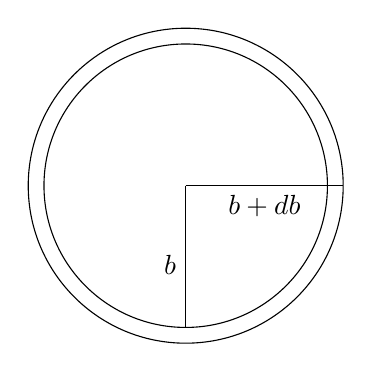
\begin{tikzpicture}
      \draw (0,0) circle [radius=2.0];
      \draw (0,0) circle [radius=1.8];
      \draw (0,0) -- (1,0) node[anchor=north] {\( b + db \)} -- (2,0);
      \draw (0,0) -- (0,-1.0) node[anchor=east] {\( b \)} -- (0,-1.8);
    \end{tikzpicture}
  \end{center}
  \caption{The ring whose area represents the possible region in which alpha
    particles may be incident on a target nucleus.}
  \label{fig:crossSecRing}
\end{figure}

The area of this ring is found as the area of any ring is found:

\begin{align*}
  A &= \pi (b + db)^2 - \pi b^2 \\
    &= \pi (b^2 + 2 b db + db^2) - \pi b^2 \\
    &= \pi b^2 + 2 \pi b db + \pi db^2 - \pi b^2 \\
    &= 2 \pi b db + \pi db^2 \\
\end{align*}

Since \( db \) is infinitesimally small, it can be approximated to be
zero. Therefore, the area of the incident ring, \( \Delta \sigma \), is

\begin{equation}
  \Delta \sigma = 2 \pi b db
\end{equation}
\label{eqn:deltaSigma}

%\qq Since \( \Delta \sigma \) is the area of the full incident ring, an
%infinitesimal angular portion of that ring, \( d\phi \), may be represented by
%\( \Delta \sigma (\phi) = b db d\phi \). Additionally, because the impact
%parameter \( b \) is related to the scattering angle \( \theta \), \( \Delta
%\sigma \) is also a function of \( \theta \). Hence,
%
%\begin{equation*}
%  \Delta \sigma (\theta, \phi) = b db d\phi
%\end{equation*}

\qq Since the impact parameter \( b \) is directly proportional to the size of
the cross section and the scattering angle \( \theta \) is inversely
proportional to the impact parameter, the size of the cross section decreases as
the scattering angle increases. Therefore, the cross section experiences a
negative rate of change as \( \theta \) increases. Hence,

\begin{equation}
  \Delta \sigma (\theta) = - d\sigma (\theta)
\end{equation}
\label{eqn:dSigma}

\qq The circumference of a circle is equal to \( 2 \pi r \), where \( r \) is
the radius of the circle. In the experiment, the radius of the ring onto which
the alpha particle is projected after it is scattered is \( R \sin{(\theta)} \),
where \( \theta \) is the scattering angle and \( R \), described in Figure
\ref{fig:alphaDist}, is the distance between the point at which the alpha
particle was scattered and the edge of the ring.

\begin{figure}[H]
  \begin{center}
    \begin{tikzpicture}

      % nucleus
      \fill (0,0) circle (2pt) node[anchor=north] {nucleus};
      \draw [dotted] (0,0) -- (0,2);

      % axis
      \draw [thick] (-2,0) -- (5,0);

      % circle
      \draw (4,1.5) -- (4,-1.5);
      \draw [dotted] (4,1.5) -- (4,2);

      % particle path
      \draw [dashed] (-1,0.5) -- (-0.5,0.5);
      \draw [dashed] (-0.5,0.5) arc[start angle=0, end angle=20] --
      (0.5,0.7) arc[start angle=20, end angle=60];
      \draw [dashed] (0.5,0.7) -- (4,1.5);
      \draw (2,1.4) node[rotate=15] {R};

    \end{tikzpicture}
  \end{center}
  \caption{The path of the alpha particle as it is scattered by a nucleus. \( R
    \) is the path length between the nucleus and the ring of the solid
    angle.}
  \label{fig:alphaDist}
\end{figure}

\qq The outer circumference of this ring is \( 2 \pi R \sin{(\theta)} \). Since
the alpha particle is incident within a range whose minimum is \( \theta -
d\theta \), however, the ring has a thickness of \( R d\theta \). Since the
thickness of the ring is infinitesimal, the ring's area can be approximated to
be that of a rectangle. Therefore, the area of the ring is \( A = 2 \pi R
\sin{(\theta)} R d\theta \).

\qq The solid angle of the scattered alpha particles at an angle \( \theta \)
is:

\begin{align*}
  \Delta \Omega &= \frac{A}{R^2} \\
                &= \frac{(2 \pi R \sin{(\theta)} R d\theta)}{R^2} \\
\end{align*}

\begin{equation}
  d\Omega = 2 \pi \sin{(\theta)}
\end{equation}
\label{eqn:dOmega}

\qq An expression for the differential cross section \( \frac{d\sigma}{d\Omega}
(\theta) \) can be found by multiplying Equation \ref{eqn:dSigma} by Equation
\ref{eqn:dOmega} divided by itself.

\begin{align*}
  \Delta \sigma &=- \frac{d\sigma}{d\Omega} (\theta) d\Omega \\
                &= - \frac{d\sigma}{d\Omega} (\theta) 2 \pi
                  \sin{(\theta)} d\theta \\
\end{align*}

From Equation \ref{eqn:deltaSigma}:

\begin{align*}
  - \frac{d\sigma}{d\Omega} (\theta) 2 \pi \sin{(\theta)} d\theta &= 2 \pi b db
  \\
\end{align*}

\begin{equation}
  \frac{d\sigma}{d\Omega} (\theta) =
  - \frac{b}{\sin{(\theta)}} \frac{db}{d\theta}
\end{equation}
\label{eqn:diffCrossSecB}

Since it is known that \( b = \frac{Z Z^{\prime} e^2}{2 E}
\text{cot} \left( \frac{\theta}{2} \right) \), it can be inserted into Equation
\ref{eqn:diffCrossSecB}. Furthermore, since \( b \) is a function of \( \theta
\), \( \frac{db}{d\theta} \) can also be found:

\begin{align*}
  b &= \frac{Z Z^{\prime} e^2}{2 E} \text{cot} \left( \frac{\theta}{2} \right)
  \\
  \frac{db}{d\theta} &= \frac{Z Z^{\prime} e^2}{2 E}
                       \left( - \frac{1}{2} \text{csc}^2 \left( \frac{\theta}{2}
                       \right) \right) \\
  \frac{db}{d\theta} &= - \frac{Z Z^{\prime} e^2}{4 E} \text{csc}^2 \left(
                       \frac{\theta}{2} \right) \\
\end{align*}

\qq Now that \( b \) and \( db \) have been found, the full expression for the
differential cross section \( \frac{d\sigma}{d\Omega} \) can be determined:

\begin{align*}
  \frac{d\sigma}{d\Omega} (\theta)
  &= - \frac{b}{\sin{(\theta)}} \frac{db}{d\theta} \\
  &= - \left( \frac{Z Z^{\prime} e^2}{2 E} \text{cot} \left( \frac{\theta}{2}
    \right) \right)
    \frac{1}{\sin{(\theta)}}
    \left( - \frac{Z Z^{\prime} e^2}{4 E} \text{csc}^2 \left( \frac{\theta}{2}
    \right) \right) \\
  &= 2 \left( \frac{Z Z^{\prime} e^2}{4 E} \right)^2
    \frac{\cos{\left( \frac{\theta}{2} \right)}}{\sin{\left(
    \frac{\theta}{2} \right)}}
    \frac{1}{\sin{(\theta)}}
    \frac{1}{\sin^2 \left( \frac{\theta}{2} \right)} \\
  &= 2 \left( \frac{Z Z^{\prime} e^2}{4 E} \right)^2
    \cos{\left( \frac{\theta}{2} \right)}
    \frac{1}{\left( 2 \sin{\left( \frac{\theta}{2} \right)} \cos{\left(
    \frac{\theta}{2} \right)} \right)}
    \frac{1}{\sin^3 \left( \frac{\theta}{2} \right)} \\
\end{align*}

\begin{equation}
  \frac{d\sigma}{d\Omega} (\theta) = \left( \frac{Z Z^{\prime} e^2}{4 E}
  \right)^2 \frac{1}{\sin^4 \left( \frac{\theta}{2} \right)}
\end{equation}
\label{eqn:diffCrossSec}

Equation \ref{eqn:diffCrossSec} is the equation for calculating the
theoretical differential cross-section.

\qq The differential cross-section can also be found experimentally using a measured alpha particle scattering rate at a particular angle \( \theta \). First,
this relation must be constructed. The collimated beam of alpha particles begins
its journey with an incident rate of \( \frac{dN_0}{dt} \). This beam is then
incident on a thin foil with an atomic density of
\( n = \frac{\rho N_A d}{A} \), where \( \rho \) is the density of the foil
material, \( d \) is the thickness of the foil, and \( A \) is the atomic number
of the foil material. Being incident on the foil, the alpha particles are
exposed to a differential cross-section at the particular angle of
\( \frac{d\sigma}{d\Omega} (\theta) \). The alpha particles are scattered by the
nuclei across a solid angle \( \Delta \Omega = {A_{\text{detector}}}{r^2} \),
where \( A_{\text{detector}} \) is the area of the detector and \( r \) is the
distance between the foil and detector. Multiplying these factors together
results in the scattering rate of the alpha particles incident on a particular
foil at a particular angle: \( \frac{dN}{dt} (\theta) = \frac{dN_0}{dt} n
\frac{d\sigma}{d\Omega} (\theta) \Delta \Omega \). Since the scattering rate is
determined experimentally, the equation can be rearranged for the differential
cross-section:

\begin{equation}
  \frac{d\sigma}{d\Omega} (\theta) = \frac{\frac{dN}{dt}
    (\theta)}{\frac{dN_0}{dt} n \Delta \Omega}
\end{equation}
\label{eqn:expDiffCrossSec}


% Distribution of scattering function vs angle shape
\qq As you can see from equation \ref{eqn:diffCrossSec}, the angluar
dependence of the function is $\frac{1}{\sin^4 \left( \frac{\theta}{2}
  \right)}$. This implies that the curve of the function drops off
rather quickly at larger angles due to this term, therefore, the rate
drops off quickly as well.

\section{Equipment Utilized}
%List principal pieces of apparatus used by manufacturer, model and
%serial number. When it may be important, list principal
%specifications of certain pieces of equipment (e.g. the focal length
%of an optical system, etc.)

% Description of set-up in prose
\qq A series of readout electronics are used to process the signal from a photodiode detector, including: a pre-amplifier, an amplifier, a discriminator, and a counter. An oscilloscope was used to verify the signal behavior at various points in the circuit. The scattering chamber, where the Rutherford scattering process was performed, required evacuation with a vacuum pump. A rotating arm inside the chamber contains an Americium 241 source, a collimating slit, a Gold or Aluminum foil, and the photodiode. A photodiode detects the energy of the alpha particle and returns an electrical signal, which is then transmitted
through the aforementioned readout electronics. A more detailed description of the experimental process and implementation of this equipment can be found in the Procedure section of this report. The following list summarizes the pieces of equipment used and some relevant specifications:

% List of specs
\begin{itemize}
\item Rutherford scattering chamber
\item Aluminum foil in frame:  \\
      Molar mass 27 g/mol \\
      Thickness $1.50 \times 10^{-7}$ m \\
      Density $2.70 \times 10^6$ g/m$^3$
\item Gold foil in frame: \\
      Molar mass 197 g/mol \\
      Thickness $2.00 \times 10^{-8}$ m \\
      Density $1.93 \times 10^7$ g/m$^3$
\item Vacuum pump, for evacuating scattering chamber
\item Readout modules: \\
      Discriminator, Amplifier, Preamplifier, Counter
\item $ ^{241}$Americium (alpha source)
\item Oscilloscope, for monitoring signals on readout modules
\item Photodiode detector \\
	  Width $2.22 \times 10^{-3}$ m \\
	  Height $4.12 \times 10^{-3}$ m
\item Collimating slit \\
      Width 0.005 m
\end{itemize}

%Labeled sketch of the experimental setup
\begin{figure}[H]
\centering
% uncomment the line below to add image
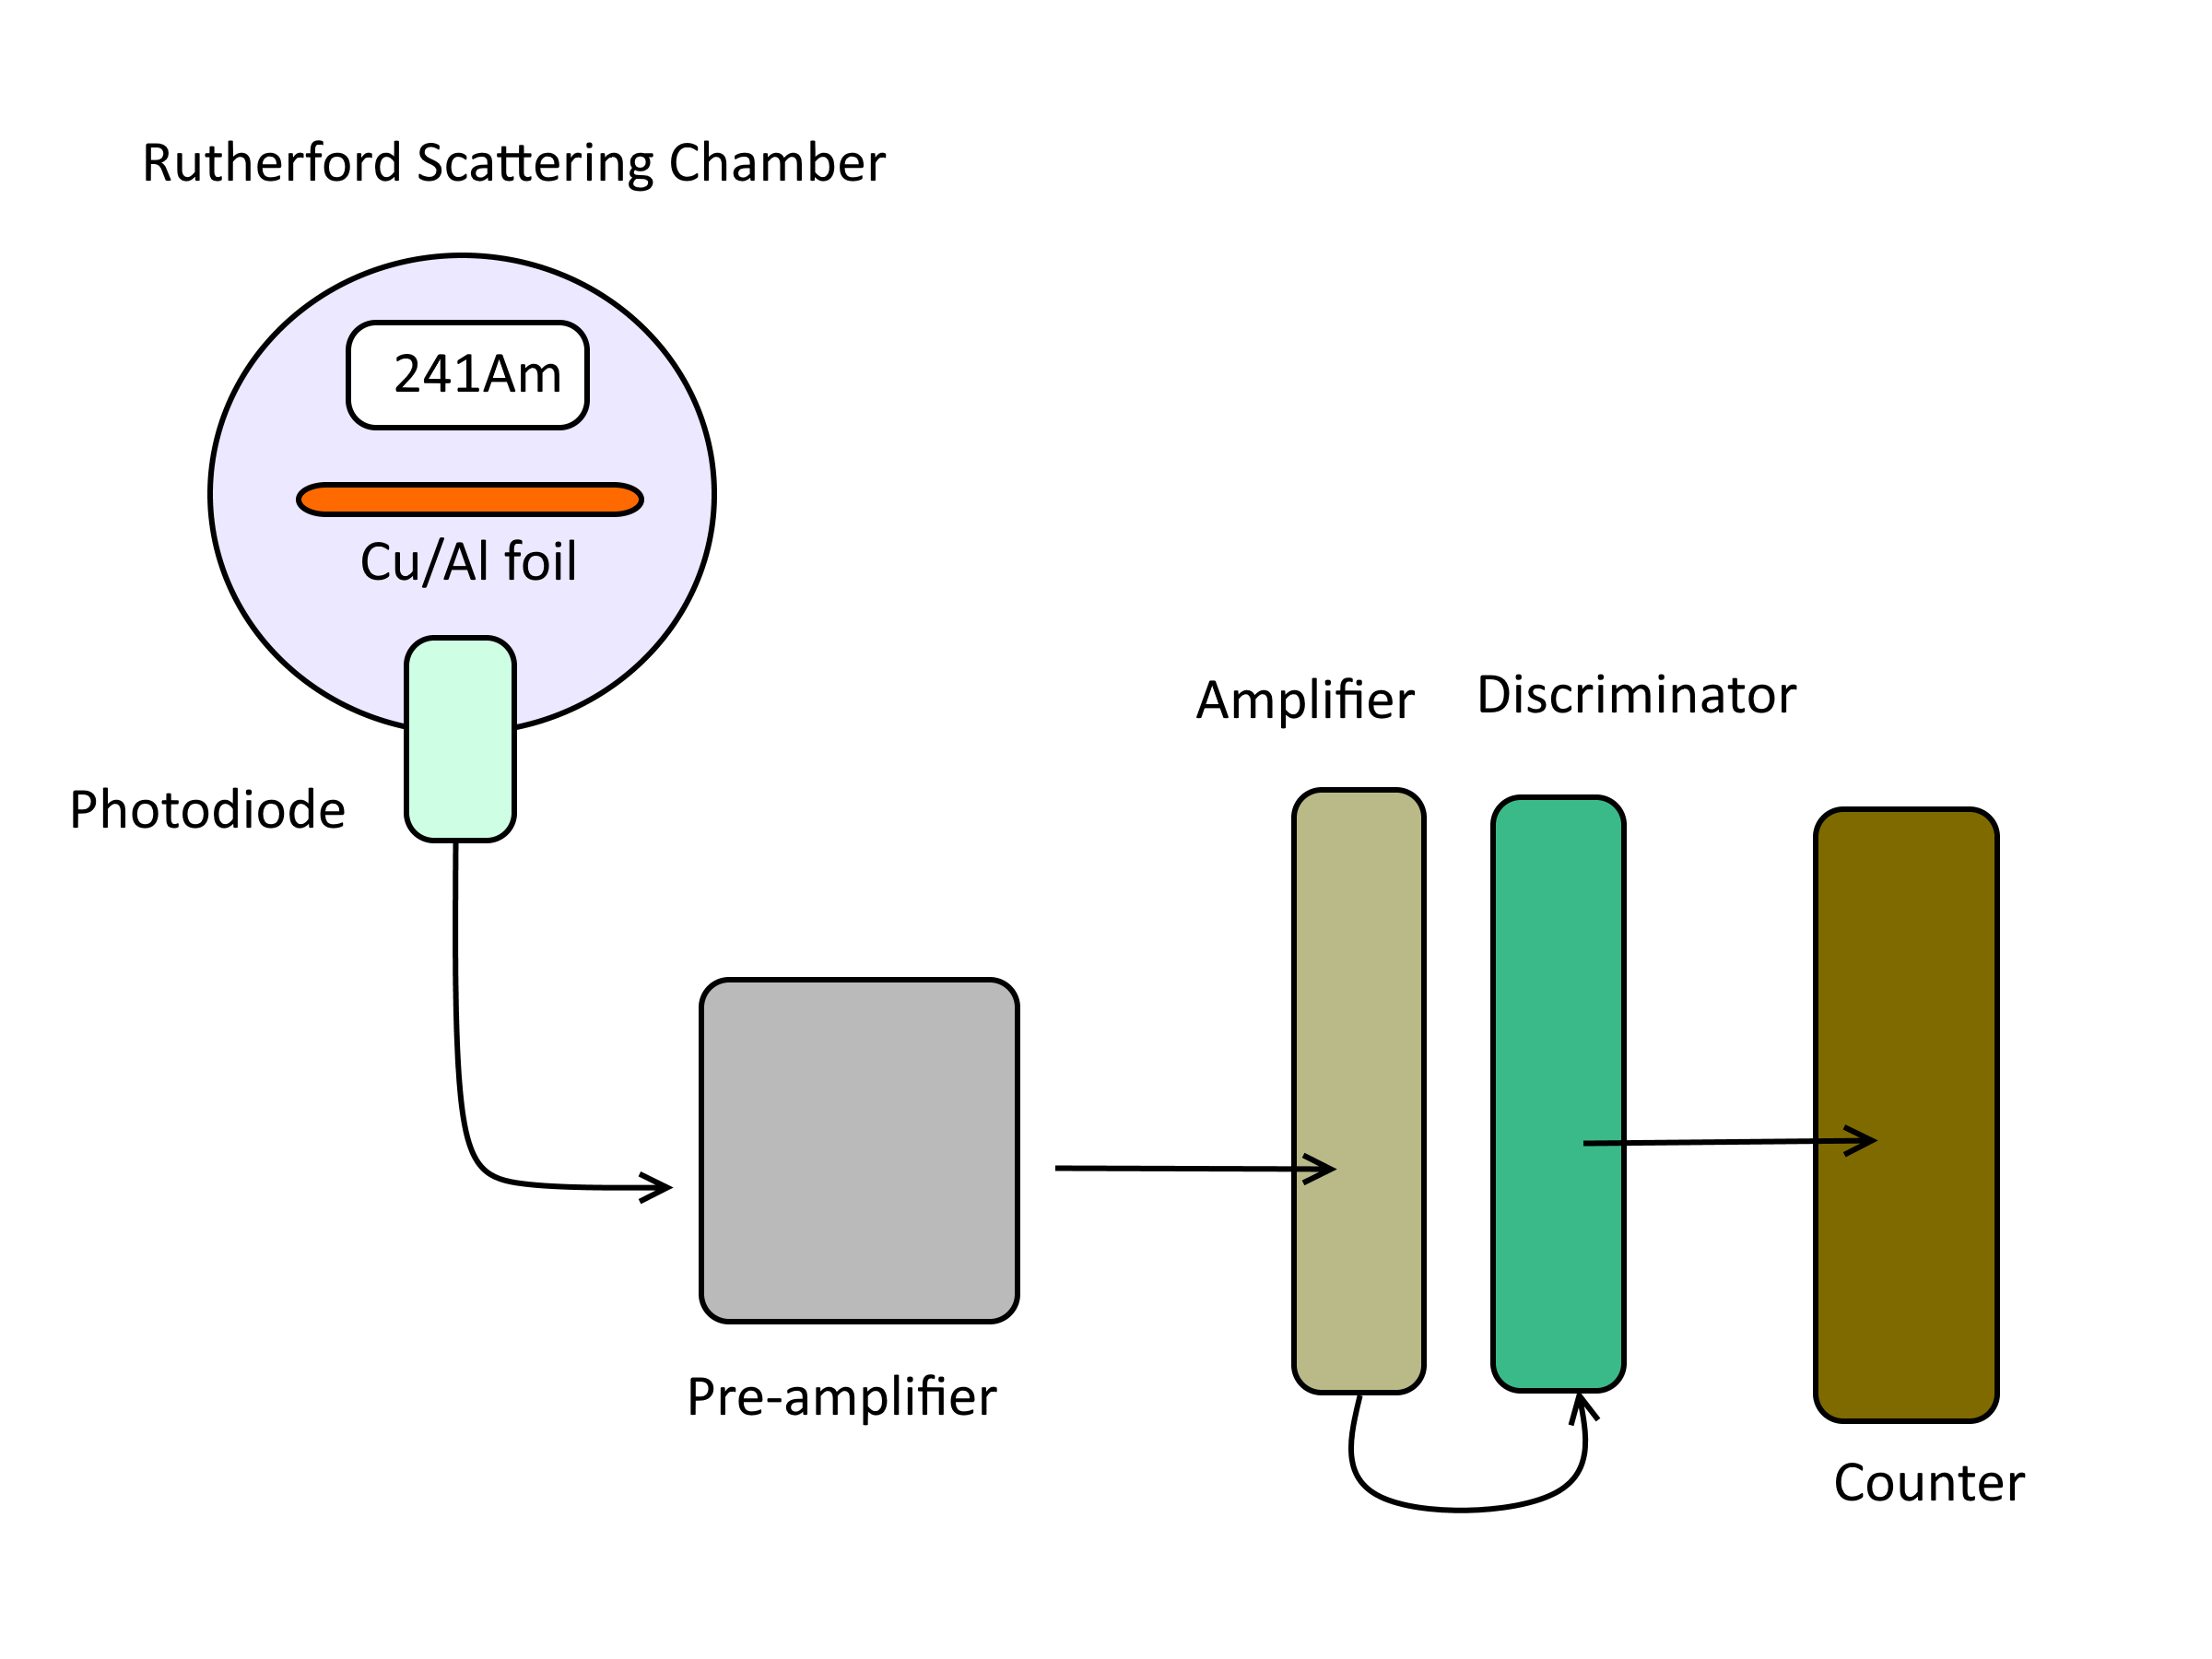
\includegraphics[width=1\textwidth]{diagram.png}
\captionof{figure}{Schematic for circuit diagram }
\label{Circuit_Diagram}
\end{figure}

\section{Procedure}

% Describe the main steps in the experimental procedures. Be sure to include any
% precautions. Sufficient details should be given such that another student can
% follow and do the experiment.

% Production in gas chamber
\qq Alpha particles are produced from an $^{241}$Am source mounted inside the
vacuum chamber on a rotating arm. Also mounted on this arm, directly in front of
the source, is a collimating slit followed by a thin gold foil. With this
configuration, one is able to strike the gold foil with a uniform, collimated
beam of alpha particles. The chamber must be evacuated using an external vacuum
pump, since alpha particles have a very short lifetime in air.

% Changing angle and measuring effect
\qq Alpha particles are scattered by Gold nuclei at varying angles, and the
scattered particles are detected using a photodiode. In order to determine the
dependence of the scattering rate on the incident angle, the rotating arm was
moved through a range of $-30$ degrees to $30$ degrees using a knob on top of
the vacuum chamber. Here, an angle of 0 degrees represents the arm oriented
along the same line as the photodiode. Because the Gold foil is
incredibly thin, any air movement resulting from the utilization of the vacuum pump can potentially damage the foil. To mitigate this risk, the pump must be opened and closed slowly. The plane of the Gold foil is also oriented parallel to the valve's tube during this process so that the foil does not impede air flow and result in a tear of the foil.

% Readout electronics
\qq The photodiode is connected via an external BNC port to a pre-amplifier that
shapes the measurement signal. This is then connected to an amplifier, which
amplifies the signal in accordance with a prescribed gain. This amplified signal
is fed to a discriminator, which sets a minimum/threshold voltage in order to
differentiate meaningful signals from electronic noise. Signals that meet this
threshold are output in the form of a digital pulse. These pulses are fed to a
counter module, which reads out the number of pulses over a given time interval.

% Acquisition time
The count rate decreases dramatically as the scattering angle increases. For
this reason, the acquisition time was increased for larger angles in order to
obtain sufficient statistics. The experimental scattering rate can be used to
calculate the differential cross-section.

\subsection{Procedural Modifications}
\qq The manual dictates that the chamber be evacuated using the vacuum pump
before conducting trials. However, it was determined that the seal of the vacuum
chamber was not sufficient, and the detected rate of alpha particles would
dramatically decrease after a few minutes. Therefore, in order to maintain a
true vacuum throughout the course of data taking, the pump was continually
operated throughout the experiment.  \qq

\subsection{Visualization of Detection Chain}
Before inserting the Gold foil, the performance of the readout electronics was investigated by observing the output of each module on an oscilloscope. The signal from the photodiode was observed via the output of the pre-amplifier. As shown in figure \ref{preamp_amp}, the signal seen on the pre-amplifier is a falling pulse. The pre-amplifier signal is then fed to the amplifier, where it undergoes a prescribed gain and is inverted. These two pulses are shown together in figure \ref{preamp_amp}. Here, the gain is set to 10, so the ampltiude of the amplifier pulse in 10 times that of the pre-amplifier pulse.

\begin{figure}[H]
\centering
% uncomment the line below to add image
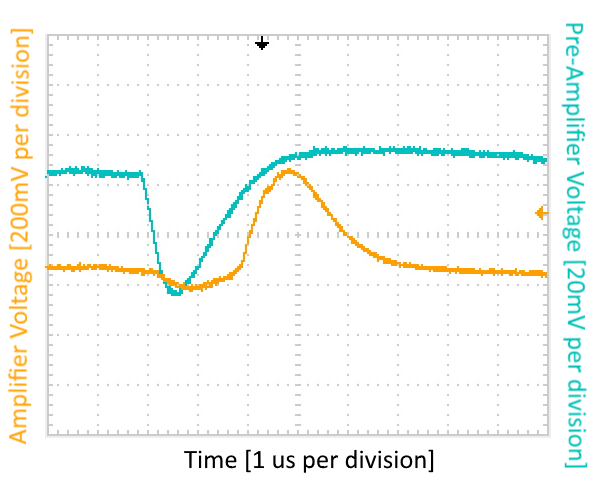
\includegraphics[width=0.7\textwidth]{gain20_th400mV_ch1amp_ch2preamp/preamp_amp.png}
\captionof{figure}{Signal pulse from the pre-amplifier and amplifier, as seen on the oscilloscope display}
\label{preamp_amp}
\end{figure}

The amplifier signal is fed to the discriminator module. If the amplifier signal has an amplitude greater than the threshold prescribed by the discriminator, then the discriminator outputs a digital pule. Figure \ref{preamp_discrim} shows this digital discriminator pulse displayed over the pre-amplifier pulse. Every pulse output by the discriminator corresponds to a count on the counter module.

\begin{figure}[H]
\centering
% uncomment the line below to add image
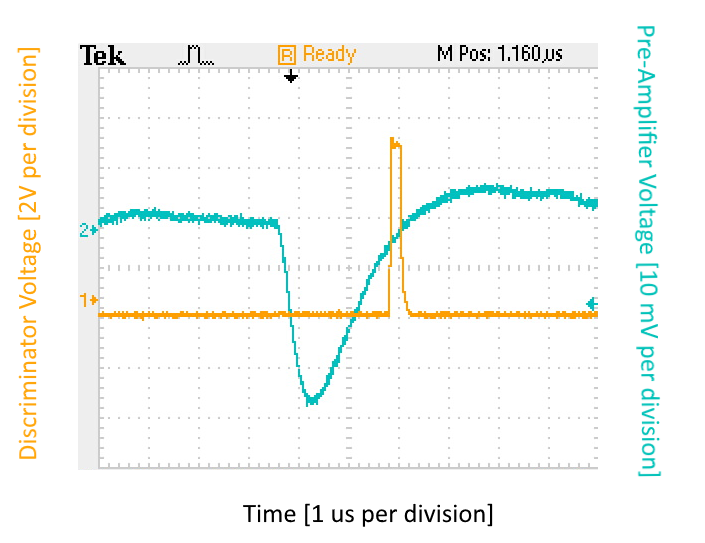
\includegraphics[width=0.75\textwidth]{ch2preamp_ch1discrim_gain20_maybe4mVthreshold/preamp_discrim.png}
\captionof{figure}{Signal pulse from the pre-amplifier and discriminator, as seen on the oscilloscope display}
\label{preamp_discrim}
\end{figure}

\section{Data Analysis}

\subsection{Data Analysis I: Gold}
%Graphs, figures, and tables with captions
%Results with error analysis
%Calculate discrepancies from theory

\subsubsection{Scattering Rate}

% Direct counting rate as a function of angle (gold)
\qq While performing the experiment, the direct rate of scattered alpha
particles for a particular angle over a certain period of time was determined
from data straight from the counter. The direct rate, \( N_d (\theta) \), was
determined simply by dividing the mean number of counts by the number of seconds
the counter was allowed to run. For the gold foil at an angle of
\( \theta = \SI{15}{\degree} \) and a time of \( t = \SI{100}{\second} \), the
direct rate was:

\begin{align*}
  N_d (\SI{15}{\degree}) &= \frac{n_m}{t} \\
  N_d (\SI{15}{\degree}) &= \frac{(1.2)}{(100)} \\
  N_d (\SI{15}{\degree}) &= \num{0.012} \\
\end{align*}

Similar calculations were performed for the remaining angles, and the results of
those calculations, as well as the collected data, can be viewed in Figure
\ref{tab:scatRatesGold}.

% Corrected counting rate (wrt. distribution in space)
\qq The direct scattering rate \( N_d (\theta) \), however, is only relevant to
a two-dimensional plane scattering geometry, not the sought-after
three-dimensional geometry. Therefore, \( N_d (\theta) \) must be extrapolated
into three dimensions. In three dimensions, the alpha particles are scattered
across a solid angle \( d\Omega \) rather than across a two-dimensional
plane. In order to take into account the third dimension, the direct scattering
rate must be multiplied by the scattering angle. The result is the spacial
scattering rate \( N (\theta) \):

\begin{align*}
  N (\theta) &= d\Omega N_d (\theta) \\
  N (\theta) &= 2 \pi \sin{(\theta)} N_d (\theta) \\
\end{align*}

\qq For the gold foil, a direct scattering rate of \( N_d (\SI{15}{\degree}) =
\num{0.012} \) yields a spacial scattering rate of:

\begin{align*}
  N (\SI{15}{\degree}) &= 2 \pi \sin{(\SI{15}{\degree})} (\num{0.012}) \\
  N (\SI{15}{\degree}) &= \num{0.0195} \\
\end{align*}

Similar calculations were performed for the remaining angles, and the results of
those calculations can be viewed in Figure \ref{tab:scatRatesGold}. The
uncertainties in the scattering rates were found by executing the Julia program
displayed in Section \ref{cod:uncertScatRateGold}.

% Experimental results for rutherford formula
\begin{figure}[H]
  \begin{center}
    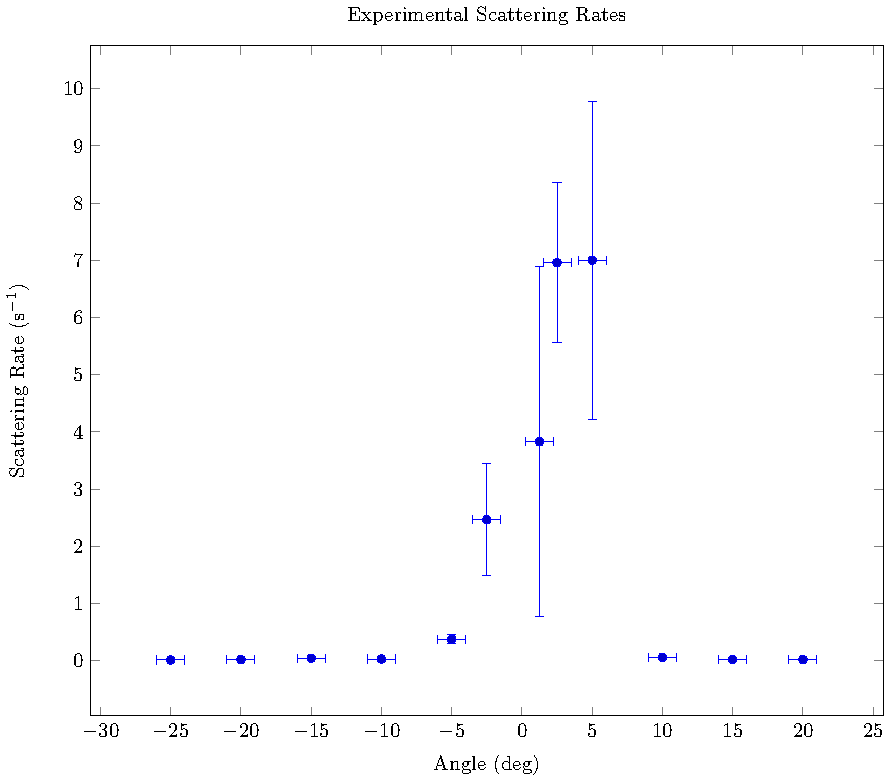
\includegraphics[scale=0.8]{Plots/ExperimentalScatteringRates/expScatRates.pdf}
  \end{center}
  \caption{The plot of the experimental values for the scattering rates of the
    alpha particles through the foil measured at different angles.}
  \label{gph:expScatRatesGold}
\end{figure}

% Experimental uncertainty (\delta)
\qq

% Theoretical results for rutherford formula
\qq The theoretical values for the scattering rates of the alpha particles
through the gold foil were determined using Rutherford's scattering formula, \(
N (\theta) = N_0 n \frac{Z^2 e^4}{(8 \pi \epsilon_0 E_{\alpha})^2 \sin^4
  \left( \frac{\theta}{2} \right)} \), where \( N_0 \) is the incident particle
rate, \( n \) is the nuclear density of the foil (found by multiplying the
foil material's atomic concentration by the foil's thickness), \( Z \) is the
nuclear number of the foil's material, \( E_{\alpha} \) is the energy of the
incident alpha particles, \( e \) is the elementary charge, and \( \epsilon_0 \)
is the dielectric constant. This formula is implemented on line 101 of the
general functions source file found in Section \ref{cod:genFuncs}. The results
of this calculation can be seen in Figure \ref{tab:scatRatesGold}.

\begin{figure}[H]
  \begin{center}
    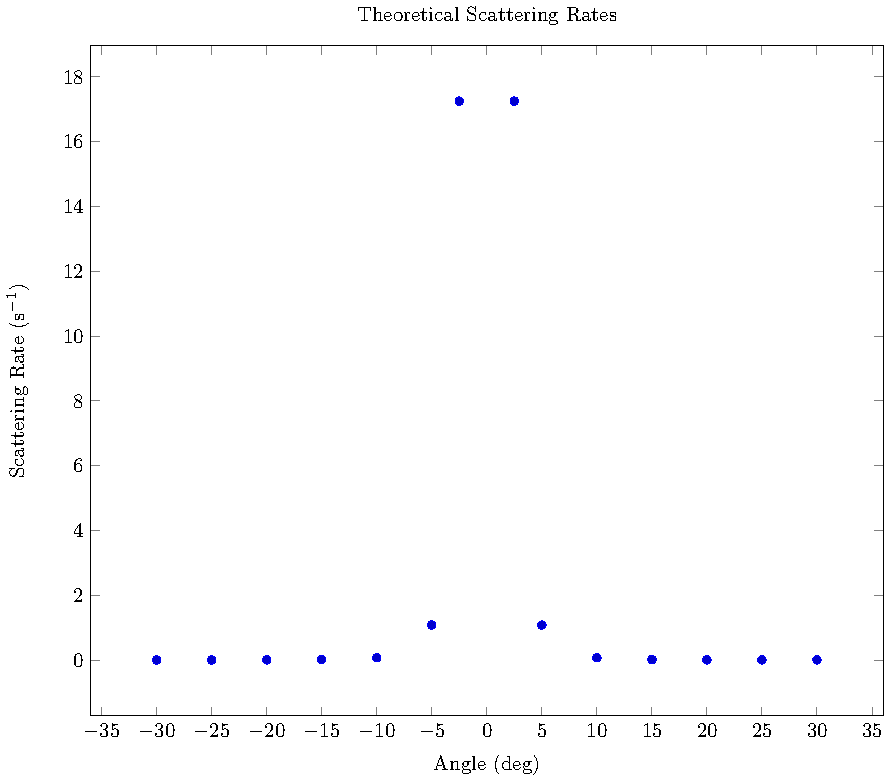
\includegraphics[scale=0.8]{Plots/TheoreticalScatteringRates/theoScatRates.pdf}
  \end{center}
  \caption{The plot of the theoretical values for the scattering rates of the
    alpha particles through the foil at different angles.}
  \label{gph:theoScatRatesGold}
\end{figure}

\subsubsection{Differential Cross Section}

\qq The equation for finding the theoretical value of the differential
cross-section is Equation \ref{eqn:diffCrossSec},
\( \frac{d\sigma}{d\Omega} (\theta) = \left( \frac{Z Z^{\prime} e^2}{4 \pi
    \epsilon_0} \right)^2 \left( \frac{1}{4 E_{\alpha}} \right)^2
\frac{1}{\sin^4 \left( \frac{\theta}{2} \right)} \). The theoretical differential
cross-section of an alpha particle emitted from an Americium-241 source
incident on a gold nucleus at \SI{15}{\degree} may be calculated in the
following manner:

\begin{align*}
  \frac{d\sigma}{d\Omega} (\theta) &= \left( \frac{Z Z^{\prime} e^2}{4 \pi
                                     \epsilon_0} \right)^2 \left( \frac{1}{4 E_{\alpha}} \right)^2
                                     \frac{1}{\sin^4 \left( \frac{\theta}{2} \right)} \\
  \frac{d\sigma}{d\Omega} (\SI{15}{\degree}) 
                                   &= \left( \frac{(79) (2) e^2}{4 \pi \epsilon_0} \right)^2 
                                     \left( \frac{1}{4 (\SI{8.79e-13}{\joule})} \right)^2
                                     \frac{1}{\sin^4 \left( \frac{(\SI{15}{\degree})}{2} \right)} \\
  \frac{d\sigma}{d\Omega} (\SI{15}{\degree}) &=
                                               \SI{239.6}{\barn\per\steradian}
  \\
\end{align*}

Similar calculations were performed for the other incident angles using the
Julia function found on line 110 in Section \ref{cod:genFuncs}, and the
results are displayed in Figure \ref{gph:theoCrossSecAu}.

\begin{figure}[H]
  \begin{center}
    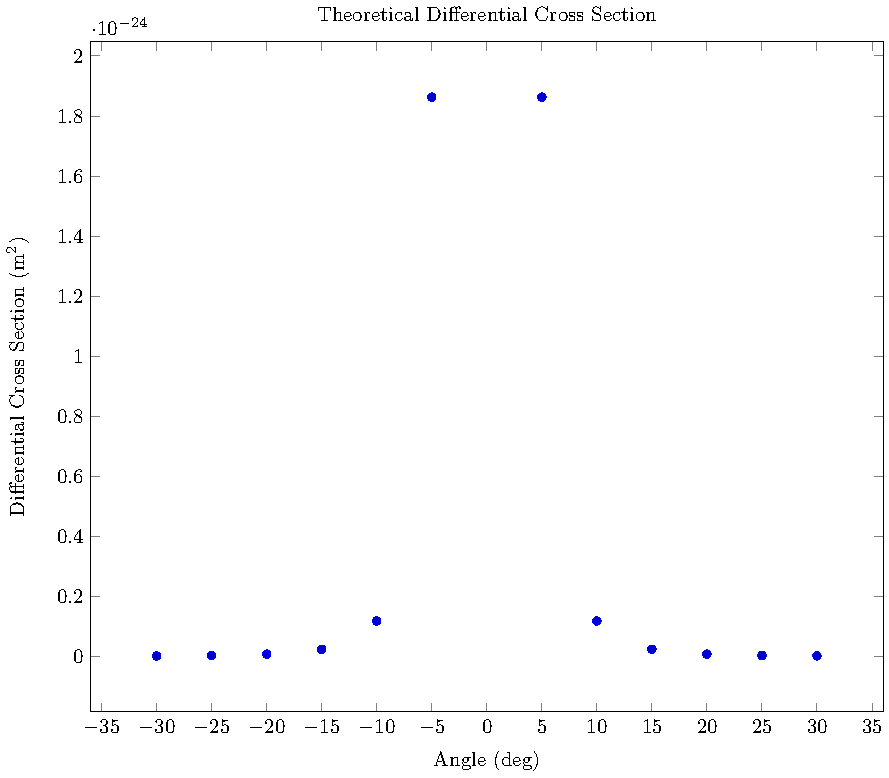
\includegraphics[scale=0.8]{Plots/TheoreticalCrossSectionalArea/theoCrossSec.pdf}
  \end{center}
  \caption{The theoretical values of the differential cross section of
    alpha particles incident on a gold nucleus at several angles.}
  \label{gph:theoCrossSecAu}
\end{figure}
  
\qq The equation for finding the experimental value of the differential
cross-section is Equation \ref{eqn:expDiffCrossSec}, \( \frac{d\sigma}{d\Omega}
(\theta) = \frac{\frac{dN}{dt} (\theta)}{\frac{dN_0}{dt} n \Delta \Omega}
\). Information collected for \( \theta = \SI{15}{\degree} \) was used to
perform the calculation.

\begin{align*}
  \frac{d\sigma}{d\Omega} (\theta) &= \frac{\frac{dN}{dt}
                                     (\theta)}{\frac{dN_0}{dt} n \Delta \Omega}
  \\
  \frac{d\sigma}{d\Omega} (\SI{15}{\degree}) 
   &= \frac{(\num{0.0195})}{(30.8) (\num{1.18e21}) (}
\end{align*}

\subsection{Data Analysis II: Aluminum}
%Graphs, figures, and tables with captions
%Results with error analysis
%Calculate discrepancies from theory

\subsubsection{Scattering Rate}

\qq The nuclear charge number of aluminum can be determined with \\
\( Z_{\text{Al}} = \sqrt{\frac{N_{\text{Al}} (\theta) n_{\text{Al}}
    Z^2_{\text{Al}}}{N_{\text{Au}} (\theta) n_{\text{Au}}}} \), where
\( N_x (\theta) \) is the spacial scattering rate of alpha particles through a
foil of material \( x \) at an angle \( \theta \), \( n_x \) is the nuclear
density of the foil of material \( x \) (found by multiplying the foil
material's atomic concentration by the foil's thickness), and \( Z_x \) is the
nuclear number of material \( x \).

% Direct counting rate as a function of angle (gold)
\qq The direct counting rate and the spacial counting rate were calculated in
the same manner as for gold. The results of the experiment are displayed in
Figure \ref{tab:scatRatesAl}.

% Corrected counting rate (wrt. distribution in space)
\qq

% Experimental results for rutherford formula
\qq Since the nuclear charge formula requires the scattering rates of both gold
and aluminum, the uncertainty for both measurements needed to be propagated
through it. The uncertainty for the scattering rates through gold was calculated
in the code shown in Section \ref{cod:uncertScatRateGold}, and the uncertainty
for the scattering rates through aluminum was calculated in the code shown in
Section \ref{cod:uncertScatRateAl}. The plots for those two calculations are
shown in Figures \ref{gph:expScatRatesGold} and \ref{gph:expScatRatesAl}
respectively. The experimental value for the nuclear number of aluminum was
calculated using the code shown in Section \ref{cod:uncertNucNumAl}, and it was
determined to be \( 62.7 \pm 3.216 \).

\begin{figure}[H]
  \begin{center}
    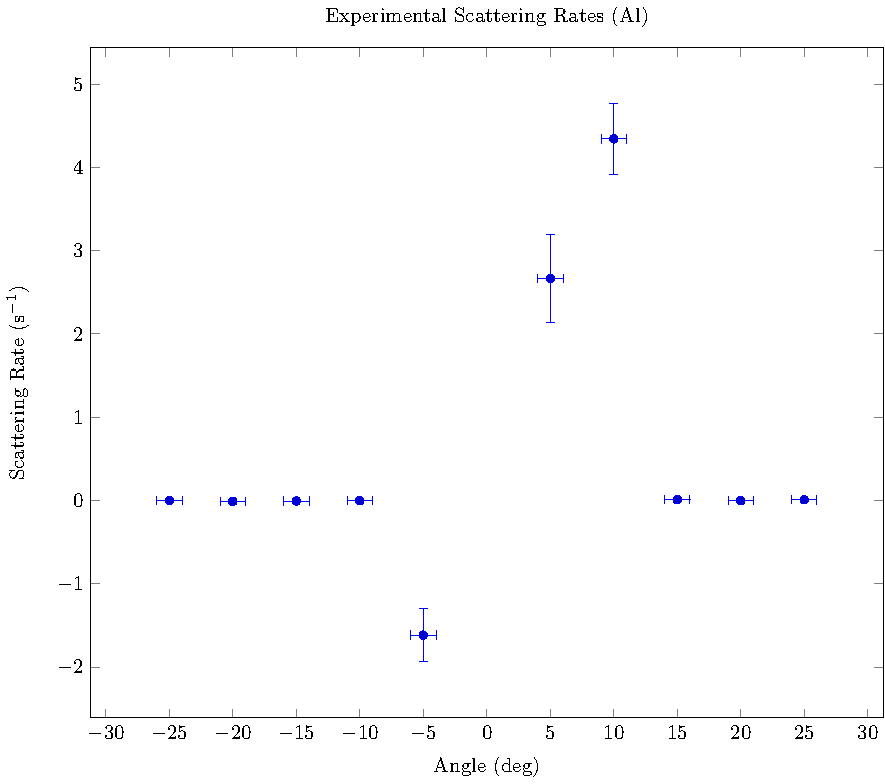
\includegraphics[scale=0.8]{Plots/ExperimentalScatteringRatesAl/expScatRatesAl.pdf}
  \end{center}
  \caption{The plot for the experimental scattering rates of alpha particles
    through an aluminum foil.}
  \label{gph:expScatRatesAl}
\end{figure}

% Experimental uncertainty (\delta)
\qq

% Theoretical results for rutherford formula
\qq The theoretical value of aluminum's nuclear charge was calculated in much
the same way as the experimental, except the theoretical values of the
scattering rates of the two foils were used. The theoretical values of the
scattering rates through both gold and aluminum were calculated using the code
shown in Sections \ref{cod:theoScatRateGold} and \ref{cod:theoScatRateAl}
respectively, and the data is represented graphically in Figures
\ref{gph:theoScatRateGold} and \ref{gph:theoScatRateAl}. The theoretical value
of the aluminum's nuclear charge was calculated using the code shown in Section
\ref{cod:theoNucNumAl}, and it's value was found to be 13.

\begin{figure}[H]
  \begin{center}
    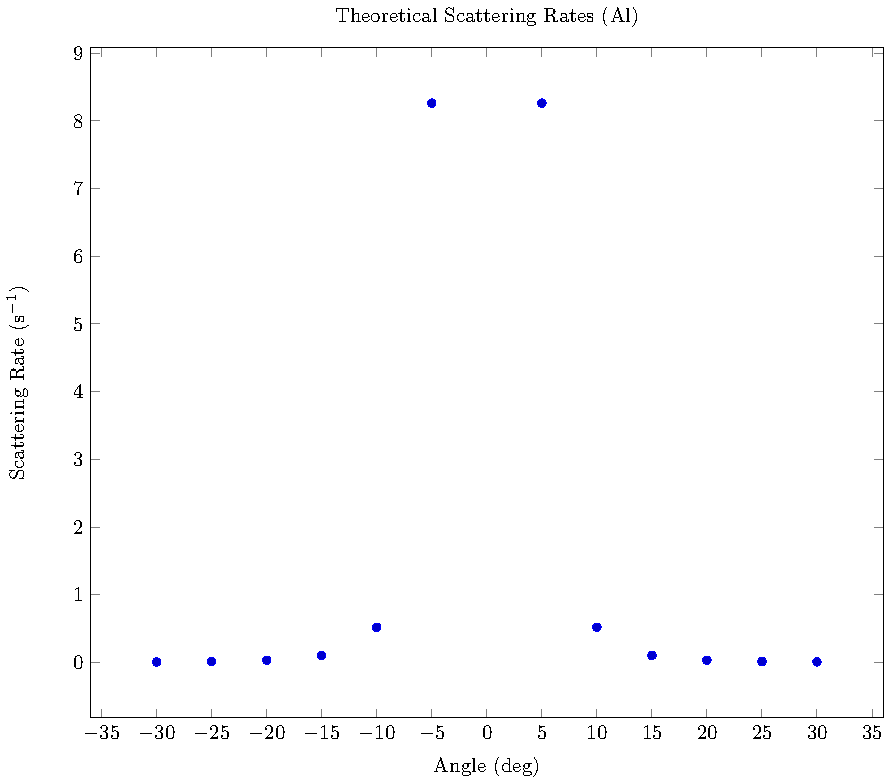
\includegraphics[scale=0.8]{Plots/TheoreticalScatteringRatesAl/theoScatRatesAl.pdf}
  \end{center}
  \caption{The plot for the theoretical scattering rates of alpha particles
    through an aluminum foil.}
  \label{gph:theoScatRateAl}
\end{figure}

\section{Results}

\subsection{Results I: Gold}
%Discuss results and uncertainties
%Compare results with theory
%Approximations to theory

% Tabulate theo and exp values/uncertainties
\qq

% Calculate the difference/discrepancy (\Delta)
\qq

% Calculate the uncertainty in the discrepancy
% Quantify how many sigmas the discrepancy is
\qq The differential cross-section is calculated using equation \ref{eq:expCrossSec}, shown below.

\begin{equation} \label{eq:expCrossSec}
 \frac{d \sigma}{d \Omega} = \frac
                                 {
								  \frac{dN}{dt} ( \theta )
								}
								{
								  \frac{dN_0}{dt}
								  \times n
								  \times \Delta \Omega
                                 }
\end{equation}

The uncertainty in this differential cross-section measurement is propagated as follows:
\begin{equation} \label{eq:expCrossSecUncert}
 \delta \left( \frac{d \sigma}{d \Omega} \right)
   = \left\lvert \frac{d \sigma}{d \Omega} \right\rvert
   \sqrt
   {
        \left( \frac{\delta dN/dt}{dN/dt} \right) ^2
        +
        \left( \frac{\delta dN_0/dt}{dN_0/dt} \right) ^2
        +
        \left( \frac{\delta n}{n} \right) ^2
        +
        \left( \frac{\delta \Delta \Omega}{\Delta \Omega} \right) ^2
   }
\end{equation}
Note that in equation \ref{eq:expCrossSecUncert}, $\delta dN/dt$ and $\delta dN_0/dt$ are uncertainties in measured rates, $n$ is a given value that can be assumed to have no uncertainty, and $\delta \Delta \Omega$ is propagated from the distance to the photodiode and the height and width of the photodiode windows as follows:
\begin{align*}
\Delta \Omega &= \frac{A}{r^2} \\
              &= \frac{h \times w}{r^2} \\
              &= \frac{(4.12 \times 10^{-3}m) \times (2.22 \times 10^{-3}m)}{(1.97 \times 10^{-2} m)^2} \\
              &= 0.02 \text{ sterad}
\end{align*}
The uncertainties in the height, width, and distance were taken to be the standard deviation of a set of three measurements taken for each quantity.
\begin{align*}
 \delta \left( \Delta \Omega  \right)
   &= | \Delta \Omega |
   \sqrt{
        \left( \frac{\delta h}{h} \right) ^2
        +
         \left( \frac{\delta w}{w} \right) ^2
        + 2 \left( \frac{\delta r}{r} \right) ^2
   } \\
   &= | 0.02 \text{ sterad} |
   \sqrt{
        \left( \frac{4.75 \times 10^{-4}}{4.12 \times 10^{-3}} \right) ^2
        +
         \left( \frac{7.64 \times 10^{-5}}{2.22 \times 10^{-3}} \right) ^2
        + 2 \left( \frac{5.01 \times 10^{-4}}{1.97 \times 10^{-2}} \right) ^2
   } \\
   &= 0.0025 \text{ sterad}
\end{align*}

The difference between experimental and theoretical cross-section values has an associated uncertainty. If the theoretical value is assumed to have no uncertainty, then the uncertainty associated with the difference will be that calculated in equation \ref{eq:expCrossSecUncert}.

\subsection{Results II: Aluminum}
%Discuss results and uncertainties
%Compare results with theory
%Approximations to theory

% Tabulate theo and exp values/uncertainties
\qq

% Calculate the difference/discrepancy (\Delta)
\qq

% Calculate the uncertainty in the discrepancy
% Quantify how many sigmas the discrepancy is
\qq

\subsection{Source of Error}
% Describe sources of error, what type of error they are, and how they
%would affect measurements (what we did about them if possible)
%i.e. leaky vacuum would kill off alphas and systematically lower
%rate, but we kept pump on to mitigate this i.e. if threshold was too
%low we would have "false counts" which would systematically increase
%rate. Note that our baseline noise seemed to increase on last day
%without changing any other factors, an d we're not sure of the source
%but we thinking maybe bad cable connection, but we had to reassess
%the baseline noise and increase threshold. BUT signal-to-noise ration
%was still sufficiently high that increasing threshold should not run
%risk of cutting out "real counts" Thickness of foil could be
%nonuniform -> random error Other stuff

\qq The Rutherford scattering chamber does not hold a perfect vacuum
seal when the valve is fully closed, potentially due to a bad o-ring. The closing valve also had some issues opening and closing, so for this reason it was decided that the valve would be left open and the vacuum pump left on. Alpha particles have a much shorter lifetime in air than in a vacuum. For this reason, a poor vacuum seal that allows air to enter the chamber would result in alpha particles that decay before reaching the detector, and this would systematically lower the measured count rate. Again, this issue was
combated by maintaining the vacuum inside the chamber. \\
\qq Electronic noise can systematically increase the measured rate if an appropriate threshold is not set. If the threshold is too low, higher amplitude noise could be counted as "signals". The amplitude of the baseline noise was observed, and a threshold was set to remove signals below this amplitude. On the final day of data collection, the amplitude of the background noise seemed to increase from the previous
sessions, even though no characteristics of the set-up were altered. While still unclear, it was suspected that a poor cable connection was responsible for the noise. The threshold was increased to account for this increased noise level. However, the
signal-to-noise ratio was still sufficiently high so that, even with the increased threshold, there was little risk of true counts falling below this threshold. However, if any lower energy alpha particles fell below this increased threshold, data taken on this data would show systematically lower rates due to the decreased counts. \\
\qq The rate of scattering is dependent on the area density of the
scatterers (gold nuclei), which in turn is dependent on the thickness of the foil. This parameter is assumed to be constant throughout experimentation. Any fluctuation in the thickness of the foil would therefore contribute a random intrinsic error in the
density of scatterers, and by extension in the scattering rate. 

\section{Conclusion}
%Brief summary, discussion of theory

% Results for gold
% Note the number of sigmas (discrepancy) and what that means statistically
\qq

% Results for aluminum
% Note the number of sigmas (discrepancy) and what that means statistically
\qq

\section{Appendices}

\subsection{Appendix A: Data}

\subsubsection{Gold Scattering Rates}

\begin{figure}[H]
  \caption{The found and calculated experimental and theoretical values
    pertaining to the scattering rate of alpha particles through gold foil.}
  \begin{center}
    \begin{adjustwidth}{-3.75cm}{}
      \begin{tabular}{|r|r|r|r|r|r|r|}
        \hline
        Angle (\si{\degree}) & Gate Time (\si{\second}) & Pulse Counts & Mean
                                                                         Counts &
                                                                                  Direct
                                                                                  Rate (\si{\per\second}
        & Spacial Rate (\si{\per\second}) & Theoretical Rate (\si{\per\second}) \\
      \hline
        \hline
                             & & 3 & & & & \\
        -25 & 600 & 2 & 2.5 & \num{0.00417} & \num{-0.0111} & \num{0.00178} \\
        \hline
                             & & 1 & & & & \\
                             & & 0 & & & & \\
                             & & 0 & & & & \\
                             & & 2 & & & & \\
        -20 & 200 & 5 & 1.6 & \num{0.008} & \num{-00172} & \num{0.00430} \\
        \hline
                             & & 1 & & & & \\
                             & & 0 & & & & \\
                             & & 0 & & & & \\
                             & & 11 & & & & \\
        -15 & 100 & 1 & 2.6 & \num{0026} & \num{-0.0423} & \num{0.0135} \\
        \hline
                             & & 3 & & & & \\
                             & & 1 & & & & \\
                             & & 3 & & & & \\
                             & & 3 & & & & \\
        -10 & 100 & 2 & \num{2.4} & \num{0.024} & \num{-0.0262} & \num{0.0677} \\
        \hline
                             & & 55 & & & & \\
                             & & 69 & & & & \\
                             & & 62 & & & & \\
                             & & 76 & & & & \\
        -5 & 100 & 79 & 68.2 & \num{0.682} & \num{-0.373} & \num{1.079} \\
        \hline
                             & & 876 & & & & \\
        -2.5 & 100 & 922 & 899 & 8.99 & -2.46 & 17.25 \\
        \hline
                             & & 2688 & & & & \\
        0 & 100 & 2746 & 2717 & 27.17 & 0 & \( \infty \) \\
      \hline
        2.5 & 100 & 2539 & 2539 & 25.39 & 6.96 & 17.25 \\
        \hline
                             & & 1225 & & & & \\
                             & & 1352 & & & & \\
                             & & 1263 & & & & \\
                             & & 1238 & & & & \\
        5 & 100 & 1315 & 1278.6 & 12.79 & 7.002 & 1.079 \\
        \hline
                             & & 5 & & & & \\
                             & & 8 & & & & \\
                             & & 4 & & & & \\
                             & & 7 & & & & \\
        10 & 100 & 3 & 5.4 & \num{0.054} & \num{0.0589} & \num{0.0677} \\
        \hline
                             & & 1 & & & & \\
                             & & 3 & & & & \\
                             & & 1 & & & & \\
                             & & 0 & & & & \\
        15 & 100 & 1 & 1.2 & \num{0.012} & \num{0.0195} & \num{0.0135} \\
        \hline
      \end{tabular}
    \end{adjustwidth}
  \end{center}
  \label{tab:scatRatesGold}
\end{figure}

  \begin{figure}[H]\ContinuedFloat
    \begin{center}
      \begin{adjustwidth}{-3.75cm}{}
        \begin{tabular}{|r|r|r|r|r|r|r|}
          \hline
          Angle (\si{\degree}) & Gate Time (\si{\second}) & Pulse Counts & Mean
                                                                           Counts &
                                                                                    Direct
                                                                                    Rate
                                                                                    (\si{\per\second})
          & Spacial Rate (\si{\per\second}) & Theoretical Rate (\si{\per\second}) \\
          \hline
          \hline
          & & 0 & & & & \\
          & & 0 & & & & \\
          & & 0 & & & & \\
          & & 6 & & & & \\
          20 & 200 & 2 & 1.6 & \num{0.008} & \num{0.0172} & \num{0.00430} \\
          \hline
          & & 0 & & & & \\
          25 & 600 & 2 & 1 & \num{0.00167} & \num{0.00443} & \num{0.00178} \\
          \hline
        \end{tabular}
      \end{adjustwidth}
    \end{center}
  \end{figure}

\subsubsection{Scattering Rates Aluminum}

\begin{figure}[H]
  \caption{The collected and calculated experimental and theoretical data
    pertaining to the scattering rates of the alpha particles at different
    angles through the aluminum foil.}
  \begin{center}
    \begin{adjustwidth}{-3.75cm}{}
      \begin{tabular}{|r|r|r|r|r|r|r|}
        \hline
        Angle (\si{\degree}) & Gate Time (\si{\second}) & Pulse Counts & Mean
                                                                         Counts
        & Direct Rate (\si{\per\second}) & Spacial Rate (\si{\per\second}) &
                                                                             Theoretical
                                                                             Rate
                                                                             (\si{\per\second})
        \\
        \hline
        \hline
        -25 & 600 & 0 & 0 & 0 & \num{0.0136} \\
        \hline
        -20 & 200 & 1 & 1 & \num{0.005} & \num{-0.0107} & \num{0.0329} \\
        \hline
                             & & 0 & & & & \\
                             & & 1 & & & & \\
        -15 & 100 & 0 & \num{0.333} & \num{0.333} & \num{-0.00542} &
                                                                     \num{0.1030}
        \\
        \hline
        & & 0 & & & & \\
        -10 & 100 & 0 & 0 & 0 & \num{0.518} \\
        \hline
        & & 284 & & & & \\
        & & 363 & & & & \\
        & & 302 & & & & \\
        & & 310 & & & & \\
        -5 & 100 & 216 & 295 & 2.95 & \num{-1.615} & \num{8.263} \\
        \hline
        & & 531 & & & & \\
        & & 459 & & & & \\
        & & 509 & & & & \\
        & & 470 & & & & \\
        5 & 100 & 465 & 486.8 & 4.868 & 2.666 & 8.263 \\
        \hline
        & & 3 & & & & \\
        & & 1 & & & & \\
        10 & 100 & 3 & 398 & 3.98 & 4.342 & \num{0.518} \\
        \hline
        & & 0 & & & & \\
        & & 1 & & & & \\
        15 & 100 & 1 & 0.667 & \num{0.00667} & \num{0.0108} & \num{0.103} \\
        \hline
        20 & 200 & 0 & 0 & 0 & 0 & \num{0.0329} \\
        \hline
        25 & 600 & 2 & 2 & \num{0.00333} & \num{0.00885} & \num{0.0136} \\
        \hline
      \end{tabular}
    \end{adjustwidth}
  \end{center}
  \label{tab:scatRatesAl}
\end{figure}

\subsection{Appendix B: Source Code}

%\subsubsection{General Functions}
%\label{cod:genFuncs}
%\inputminted{julia}{Code/genFuncs.jl}
%
%\subsubsection{Error Propagation for Scattering Rates through Gold}
%\label{cod:uncertScatRateGold}
%\inputminted{julia}{Code/getUncertScatRate.jl}
%
%\subsubsection{Error Propagation for Scattering Rates through Aluminum}
%\label{cod:uncertScatRateAl}
%\inputminted{julia}{Code/getUncertScatRateAl.jl}
%
%\subsubsection{Compute the Theoretical Scattering Rates through Gold}
%\label{cod:theoScatRateGold}
%\inputminted{julia}{Code/getTheoScatRatesGold.jl}
%
%\subsubsection{Compute the Theoretical Scattering Rates through Aluminum}
%\label{cod:theoScatRateAl}
%\inputminted{julia}{Code/getTheoScatRatesAl.jl}
%
%\subsubsection{Error Propagation for Differential Cross Section through Gold}
%\label{cod:uncertCrossSecAu}
%\inputminted{julia}{Code/getUncertCrossSec}

%\subsubsection{Error Propagation for Nuclear Number of Aluminum}
%\label{cod:uncertNucNumAl}
%\inputminted{julia}{Code/getUncertNucNumAl.jl}
%
%\subsubsection{Compute the Theoretical Nuclear Number of Aluminum}
%\label{cod:theoNucNumAl}
%\inputminted{julia}{Code/getTheoNucNumAl.jl}
%
\end{document}
